\documentclass[10pt]{article}

%Polytechnic Institute of Viseu
%School of Technology and Management of Viseu
%File Template Dissertation Created by Gilberto Rouxinol on 2023
%https://www.overleaf.com/
%Copyright © https://ctan.org
%Copyright © MIT License 2023 Gilberto Rouxinol


%Texto
\usepackage[utf8]{inputenc}
\usepackage[portuguese]{babel}

%Texto cor
\usepackage{xcolor}

%Bibliografia
\usepackage[backend=biber, style=numeric, sorting=ynt]{biblatex}
\addbibresource{G_RefBiblio.bib}
\usepackage{csquotes}

%Configuração da página
\usepackage[a4paper,left=3.0cm,right=3.0cm,top=2.5cm,bottom=2.5cm]{geometry}

%Alinhar equações
\usepackage{amsmath}

%Fontes ou símbolos matemáticos
\usepackage{amssymb}

%Referências de figuras
\usepackage{graphicx}

%Colocar subfiguras
\usepackage{caption}
\usepackage{subcaption}

%Escrever unidades do SI
\usepackage{siunitx}

%Acrescentar pdfs
\usepackage{pdfpages}

%Paginação
\usepackage{fancyhdr}
\pagestyle{fancy}
\fancyhf{}
\renewcommand{\headrulewidth}{0pt}
\fancyfoot[R]{\thepage}

%Criar os níveis de profundidade de subsubsubsection e de subsubsubsubsection
\setcounter{secnumdepth}{5}
\makeatletter
\newcommand\subsubsubsection{\@startsection{paragraph}{4}{\z@}{-2.5ex\@plus -1ex \@minus -.25ex}{1.25ex \@plus .25ex}{\normalfont\normalsize\bfseries}}
\newcommand\subsubsubsubsection{\@startsection{subparagraph}{5}{\z@}{-2.5ex\@plus -1ex \@minus -.25ex}{1.25ex \@plus .25ex}{\normalfont\normalsize\bfseries}}
\makeatother

%Indicar o nível de profundidade do índice geral
\setcounter{tocdepth}{5}

%Renomear o nome por defeito de secções padrão
\addto\captionsportuguese{\renewcommand{\contentsname}{ÍNDICE GERAL}}
\addto\captionsportuguese{\renewcommand{\listfigurename}{ÍNDICE DE FIGURAS}}
\addto\captionsportuguese{\renewcommand{\listtablename}{ÍNDICE DE TABELAS}}

%Contemplar o nome de secções não padrão no índice geral
\addcontentsline{toc}{section}{ÍNDICE DE TABELAS}
\addcontentsline{toc}{section}{ÍNDICE DE FIGURAS}
\addcontentsline{toc}{section}{LISTA DE SIGLAS/ABREVIATURAS}
\addcontentsline{toc}{section}{LISTA DE SÍMBOLOS}

%Colocar a numeração da secção à esquerda da numeração das equações, tabelas e figuras
\numberwithin{equation}{section}
\numberwithin{table}{section}
\numberwithin{figure}{section}


\title{\textcolor{blue}{A capa e a contracapa (modelo em pdf) devem ser inseridos antes da primeira página do trabalho}}
\author{\textcolor{blue}{retirar esta página depois}}
\date{ }

\begin{document}
\maketitle %Comentar esta linha para retirar esta página
\pagenumbering{roman}

\newpage
\section*{DEDICATÓRIA}
\textcolor{blue}{Opcional}\\ %apagar esta informação
Phasellus aliquet volutpat odio. Vestibulum ante ipsum primis in faucibus orci luctus et ultrices posuere cubilia Curae; Pellentesque sit amet pede ac sem elei- fend consectetuer. Nullam elementum, urna vel imperdiet sodales, elit ipsum pharetra ligula, ac pretium ante justo a nulla.

\newpage
\section*{AGRADECIMENTOS}
Morbi luctus, wisi viverra faucibus pretium, nibh est placerat odio, nec commodo wisi enim eget quam. Quisque libero justo, consectetuer a, feugiat vitae, porttitor eu, libero. Suspendisse sed mauris vitae elit sollicitudin malesuada. Maecenas ultricies eros sit amet ante. Ut vene- natis velit. Maecenas sed mi eget dui varius euismod. Phasellus aliquet volutpat odio. Vestibulum ante ipsum primis in faucibus orci luctus et ultrices posuere cubilia Curae; Pellentesque sit amet pede ac sem elei- fend consectetuer. Nullam elementum, urna vel imperdiet sodales, elit ipsum pharetra ligula, ac pretium ante justo a nulla. Curabitur tristique arcu eu metus. Vestibulum lectus. Proin mauris. Proin eu nunc eu urna hendrerit faucibus. Aliquam auctor, pede consequat laoreet varius, eros tellus scelerisque quam, pellentesque hendrerit ipsum dolor sed augue. Nulla nec lacus.

\newpage
\section*{RESUMO}
Vivamus adipiscing. Curabitur imperdiet tempus turpis. Vivamus sapien dolor, congue venenatis, euismod eget, porta rhoncus, magna. Proin condimentum pretium enim. Fusce fringilla, libero et venenatis facilisis, eros enim cursus arcu, vitae facilisis odio augue vitae orci. Aliquam varius nibh ut odio. Sed condimentum condimentum nunc. Pellentesque eget massa. Pellentesque quis mauris. Donec ut ligula ac pede pulvinar lobortis. Pellentesque euismod. Class aptent taciti sociosqu ad litora torquent per conubia nostra, per inceptos hymenaeos. Praesent elit. Ut laoreet ornare est. Phasellus gravida vulputate nulla. Donec sit amet arcu ut sem tempor malesuada. Praesent hendrerit augue in urna. Proin enim ante, ornare vel, consequat ut, blandit in, justo. Donec felis elit, dignissim sed, sagittis ut, ullamcorper a, nulla. Aenean pharetra vulputate odio.
\vfill
\textbf{Palavras-chave:} Palavra 1; Palavra 2; Palavra 3

\newpage
\section*{ABSTRACT}
Etiam euismod. Fusce facilisis lacinia dui. Suspendisse potenti. In mi erat, cursus id, nonummy sed, ullamcorper eget, sapien. Praesent pre- tium, magna in eleifend egestas, pede pede pretium lorem, quis con- sectetuer tortor sapien facilisis magna. Mauris quis magna varius nulla scelerisque imperdiet. Aliquam non quam. Aliquam porttitor quam a lacus. Praesent vel arcu ut tortor cursus volutpat. In vitae pede quis diam bibendum placerat. Fusce elementum convallis neque. Sed dolor orci, scelerisque ac, dapibus nec, ultricies ut, mi. Duis nec dui quis leo sagittis commodo.
\vfill
\textbf{Keywords:} Keyword 1; Keyword 2; Keyword 3

\newpage
\tableofcontents

\newpage
\listoftables

\newpage
\listoffigures

\newpage
\section*{LISTA DE SIGLAS/ABREVIATURAS}
%Exemplos
\begin{flushleft}
\begin{tabular}{l p{0.6\linewidth}}
%SIGLAS
IPV      & Instituto Politécnico de Viseu\\
ESTGV    & Escola Superior de Tecnologia e Gestão de Viseu\\
\\
%ABREVIATURAS
a. C.       & antes de Cristo\\
V. S. F. F. & volte, se faz favor\\
e. g.       & \textit{exempli gratia}\\
etc.        & \textit{et cetera}\\
ibid.       & \textit{ibidem}\\
i. e.       & \textit{id est}\\
máx.        & máximo\\
mín.        & mínimo\\
fig.        & figura\\
figs.       & figuras\\
$\text{n.}^{\text{o}}$  & número\\
$\text{n.}^{\text{os}}$ & números\\
pág.        & página\\
págs.       & páginas\\
p.          & página\\
pp.         & páginas\\
A.          & autor\\
AA.         & autores
\end{tabular}
\end{flushleft}

\newpage
\section*{LISTA DE SÍMBOLOS}
%Exemplos
\section*{a) Maiúsculas Latinas}
    \begin{flushleft}
        \begin{tabular}{l p{0.8\linewidth}}
        E      & módulo de elasticidade\\
        G      & módulo de distorção
        \end{tabular}
    \end{flushleft}
    
\section*{b) Minúsculas Latinas}
    \begin{flushleft}
        \begin{tabular}{l p{0.8\linewidth}}
        b      & largura de uma secção transversal\\
        d      & altura da parte reta de uma alma\\
        h      & altura de uma secção transversal\\
        i      & raio de giração\\
        l      & comprimento\\
        r      & raio\\
        t      & espessura
        \end{tabular}
    \end{flushleft}
    
\section*{c) Maiúsculas Gregas}
    \begin{flushleft}
        \begin{tabular}{l p{0.8\linewidth}}
        $\Lambda$  & \\
        $\Xi$      & \\
        $\Phi$     & \\
        $\Psi$     & \\
        $\Pi$      & produtório\\
        $\Theta$   & \\
        $\Gamma$   & \\
        $\Delta$   & incremento\\
        $\Omega$   & área\\
        $\Sigma$   & somatório
        \end{tabular}
    \end{flushleft}
    
\section*{d) Minúsculas Gregas}
    \begin{flushleft}
        \begin{tabular}{l p{0.8\linewidth}}
        $\alpha$   & \\
        $\beta$    & \\
        $\epsilon$ & \\
        $\zeta$    & \\
        $\eta$     & \\
        $\kappa$   & \\
        $\lambda$  & \\
        $\mu$      & \\
        $\xi$      & \\
        $\rho$     & \\
        $\tau$     & tensão tangencial\\
        $\phi$     & \\
        $\psi$     & \\
        $\pi$      & pi\\
        $\theta$   & \\
        $\gamma$   & \\
        $\delta$   & deslocamnento\\
        $\omega$   & frequência\\
        $\sigma$   & tensão normal
        \end{tabular}
    \end{flushleft}
    
\section*{e) Índices Superiores Gerais}
    \begin{flushleft}
        \begin{tabular}{l p{0.8\linewidth}}
        Elem      & elemento
        \end{tabular}
    \end{flushleft}
    
\section*{f) Índices Inferiores Gerais}
    \begin{flushleft}
        \begin{tabular}{l p{0.8\linewidth}}
        i     & i-ésimo objeto\\
        CM    & centro de massa\\
        c     & compressão\\
        t     & tração
        \end{tabular}
    \end{flushleft}
    
\section*{g) Iteração}
    \begin{flushleft}
        \begin{tabular}{l p{0.8\linewidth}}
        t     & instante t
        \end{tabular}
    \end{flushleft}
    
\section*{h) Outros}
    \begin{flushleft}
        \begin{tabular}{l p{0.8\linewidth}}
        $\dot{u}$     & primeira derivada de u em ordem ao tempo\\
        $\ddot{u}$    & segunda derivada de u em ordem ao tempo
        \end{tabular}
    \end{flushleft}

\newpage
\pagenumbering{arabic}
\section{NOME DO CAPÍTULO 1}
Lorem  ipsum  dolor  sit  amet,  consectetuer  adipiscing elit. Etiam  lobortisfacilisis sem.  Nullam nec mi et neque pharetra sollicitudin. Praesent imperdietmi nec ante. Donec ullamcorper, felis non sodales \textcolor{red}{referência bibliográfica} \cite{einstein}, \textcolor{red}{referência bibliográfica} \cite{dirac}, \textcolor{red}{referência bibliográfica} \cite{latexcompanion}, \textcolor{red}{referência bibliográfica} \cite{knuthwebsite}.

\subsection{Nome da subsecção 1 do capítulo 1}
Nulla in ipsum. Praesent eros nulla, congue vitae, euismod ut, com- modo a, wisi. Pellentesque habitant morbi tristique senectus et netus et malesuada fames ac turpis egestas. Aenean nonummy magna non leo. Sed felis erat, ullamcorper in, dictum non, ultricies ut, lectus. Proin vel arcu a odio lobortis euismod. Vestibulum ante ipsum primis in fauci- bus orci luctus et ultrices posuere cubilia Curae; Proin ut est. Aliquam odio. Pellentesque massa turpis, cursus eu, euismod nec, tempor con- gue, nulla. Duis viverra gravida mauris. Cras tincidunt. Curabitur eros ligula, varius ut, pulvinar in, cursus faucibus, augue, \textcolor{red}{referência bibliográfica} \cite{knuth-fa}, \textcolor{red}{referência bibliográfica} \cite{knuth-acp}, \textcolor{red}{referência bibliográfica} \cite{ctan}.

\subsection{Nome da subsecção 2 do capítulo 1}
Lorem ipsum dolor sit amet, consectetuer adipiscing elit. Ut purus elit, vestibulum ut, placerat ac, adipiscing vitae, felis. Curabitur dictum gravida mauris. Nam arcu libero, nonummy eget, consectetuer id, vul- putate a, \textcolor{red}{referência figura} \ref{fig:circulo} magna. Donec vehicula augue eu neque. Pellentesque habitant morbi tristique senectus et netus et malesuada fames ac turpis egestas. 

\begin{figure}[!htbp]
    \centering
    
\includegraphics[scale=0.2, angle=0]{Figuras/ftimg_1318-circulo.jpg}
    \caption{Nome da figura}
    \label{fig:circulo}
\end{figure}
Mauris ut leo. Cras viverra metus rhoncus sem. Nulla et lectus vesti- bulum urna fringilla ultrices. Phasellus eu tellus sit amet tortor gravida placerat. Integer sapien est, iaculis in, pretium quis, viverra ac, nunc. Praesent eget sem vel leo ultrices bibendum. Aenean faucibus. Morbi dolor nulla, malesuada eu, pulvinar at, mollis ac, nulla. Curabitur auc- tor semper nulla. Donec varius orci eget risus. Duis nibh mi, congue eu, accumsan eleifend, sagittis quis, diam. Duis eget orci sit amet orci dignissim rutrum.

\newpage
\section{NOME DO CAPÍTULO 2}   
Nulla ac nisl. Nullam urna nulla, ullamcorper in, interdum sit amet, gra- vida ut, risus. Aenean ac enim. In luctus. Phasellus eu quam vitae turpis viverra pellentesque. Duis feugiat felis ut enim. Phasellus pharetra, sem id porttitor sodales, magna nunc aliquet nibh, nec blandit nisl mauris at pede. Suspendisse risus risus, lobortis eget, semper at, imperdiet sit amet, quam. Quisque scelerisque dapibus nibh. Nam enim. Lorem ip- sum dolor sit amet, consectetuer adipiscing elit. Nunc ut metus. Ut metus justo, auctor at, ultrices eu, sagittis ut, purus. Aliquam aliquam.

\subsection{Nome da subsecção 1 do capítulo 2}
Duis aliquet dui in est.  \textcolor{red}{referência figura} \ref{fig:3juntas} Donec eget est. Nunc lectus odio, varius at, fermentum in, accumsan non, enim. Aliquam erat volutpat. Proin sit amet nulla ut eros consectetuer cursus. Phasellus dapibus aliquam justo. Nunc laoreet. Donec consequat placerat magna. \textcolor{red}{referência figura} \ref{fig:juntos2}.

\begin{figure}[!htbp]
    \centering
    \begin{subfigure}{0.3\textwidth}
        \centering
        
\includegraphics[width=\textwidth]{Figuras/tablet1-2022.jpg}
        \caption{}
        \label{fig:juntos1}
    \end{subfigure}
    \hfill
    \begin{subfigure}{0.3\textwidth}
        \centering
        
\includegraphics[width=\textwidth]{Figuras/tablet1-2022.jpg}
        \caption{}
        \label{fig:juntos2}
    \end{subfigure}
    \hfill
    \begin{subfigure}{0.3\textwidth}
        \centering
        
\includegraphics[width=\textwidth]{Figuras/tablet1-2022.jpg}
        \caption{}
        \label{fig:juntos3}
    \end{subfigure}
    \caption{Nome geral da figura: (a) nome da figura a; (b) nome da figura b; (c) nome da figura c}
    \label{fig:3juntas}
\end{figure}

Duis pretium tincidunt justo. Sed sollicitudin vestibulum quam. Nam quis ligula. Vivamus at metus. Etiam imperdiet imperdiet pede. Aenean turpis. Fusce augue velit, scelerisque sollicitudin, dictum vitae, tempor et, pede. Donec wisi sapien, feugiat in, fermentum ut, sollicitudin adipiscing, metus.

\subsubsection{Nome da subsubsecção 1 da subsecção 1}
Blat \textcolor{red}{referência equação} \ref{eq:funcao} sed eleifend, eros sit amet faucibus elementum, urna sapien consectetuer mauris, quis egestas leo justo non risus. Morbi non felis ac libero vul- putate fringilla. Mauris libero eros, lacinia non, sodales quis, dapibus porttitor, pede. 

\begin{equation}
    f(x) =\left\{ 
    \begin{aligned}
          &0, && \forall x\in(-\infty,0] \\
          & e^{-\frac{1}{x^2}}, && \forall x\in[0,\infty) 
    \end{aligned}
    \label{eq:funcao}
    \right.
\end{equation}

Class aptent taciti sociosqu ad litora torquent per conu- bia nostra, per inceptos hymenaeos. Morbi dapibus mauris condimentum nulla. Cum sociis natoque penatibus et magnis dis parturient montes, nascetur ridiculus mus. Etiam sit amet erat. Nulla varius. Etiam tinci- dunt dui vitae turpis. Donec leo. Morbi vulputate convallis est. Integer aliquet. Pellentesque aliquet sodales urna.

\subsubsection{Nome da subsubsecção 2 da subsecção 1}
Class aptent taciti sociosqu ad litora torquent per conubia nostra, per inceptos hymenaeos. Aenean nonummy turpis id odio. Integer euismod imperdiet turpis. Ut nec leo nec diam imperdiet lacinia. Etiam eget lacus eget mi ultricies posuere. In placerat tristique tortor. Sed porta vestibulum metus. Nulla iaculis sollicitudin pede. Fusce luctus tellus in dolor. Curabitur auctor velit a sem. Morbi sapien. Class aptent taciti sociosqu ad litora torquent per conubia nostra, per inceptos hymenaeos. Donec adipiscing urna vehicula nunc. Sed ornare leo in leo. In rhoncus leo ut dui. Aenean dolor quam, volutpat nec, fringilla id, consectetuer vel, pede.

\subsection{Nome da subsecção 2 do capítulo 2}
Class aptent taciti sociosqu ad litora torquent per conubia nostra, per inceptos hymenaeos. Aenean nonummy turpis id odio. Integer euismod imperdiet turpis. Ut nec leo nec diam imperdiet lacinia. Etiam eget lacus eget mi ultricies posuere. In placerat tristique tortor. Sed porta vestibulum metus \textcolor{red}{referência tabela} \ref{tab:tabMulti}

\begin{table}[ht]
    \centering
    \caption{Nome da tabela}
    \begin{tabular}{cccc}
        \hline
        \multicolumn{2}{c}{Lado A} & \multicolumn{2}{c}{Lado B}\\
        Texto A & $\alpha$ & Texto B & $\beta$ \\
        \hline
       1  & 100 & 5 & 500 \\
       2  & 200 & 6 & 600 \\
       3  & 300 & 7 & 700 \\
       4  & 400 & 8 & 800 \\
        \hline
    \end{tabular}
    \label{tab:tabMulti}
\end{table}

Nulla iaculis sollicitudin pede. Fusce luctus tellus in dolor. Curabitur auctor velit a sem. Morbi sapien. Class aptent taciti sociosqu ad litora torquent per conubia nostra, per inceptos hymenaeos. Donec adipiscing urna vehicula nunc.

\subsection{Nome da subsecção 3 do capítulo 2}
Fusce suscipit cursus sem. Vivamus risus mi, egestas ac, imperdiet va- rius, faucibus quis, leo. Aenean tincidunt. Donec suscipit. Cras id justo quis nibh scelerisque dignissim. Aliquam sagittis elementum dolor. Aenean consectetuer justo in pede. Curabitur ullamcorper ligula nec orci. Aliquam purus turpis, aliquam id, ornare vitae, porttitor non, wisi. Maecenas luctus porta lorem. Donec vitae ligula eu ante pretium varius.

\subsubsection{Nome da subsubsecção 1 da subsecção 3}
Praesent sed neque id pede mollis rutrum. Vestibulum iaculis risus. \textcolor{red}{referencia tabela} \ref{tab:tabAB} Pellentesque lacus. Ut quis nunc sed odio malesuada egestas. Duis a ma- gna sit amet ligula tristique pretium. Ut pharetra. Vestibulum imperdiet magna nec wisi. Mauris convallis. Sed accumsan sollicitudin massa \textcolor{red}{referencia tabela} \ref{tab:tabA}

\begin{table}[h]
    \centering
    \caption{Nome geral das tabelas: (a) nome tabela A; (b) nome tabela B}
    \begin{subtable}[h]{0.4\textwidth}
        \centering
        \caption{}
        \begin{tabular}{llll}
            \hline
              & A & B & C \\
            \hline
           X  & 1 & 2 & 3 \\
           Y  & 4 & 5 & 6 \\
           Z  & 7 & 8 & 9 \\
            \hline
        \end{tabular}
        \label{tab:tabA}
    \end{subtable}
    \begin{subtable}[h]{0.4\textwidth}
        \centering
        \caption{}
        \begin{tabular}{llll}
            \hline
              & A & B & C \\
            \hline
           X  & 1 & 2 & 3 \\
           Y  & 4 & 5 & 6 \\
           Z  & 7 & 8 & 9 \\
            \hline
        \end{tabular}
        \label{tab:tabB}
    \end{subtable}
    \label{tab:tabAB}
\end{table}

Sed id enim. Nunc pede enim, lacinia ut, pulvinar quis, suscipit semper, elit. Cras accumsan erat vitae enim. Cras sollicitudin. Vestibulum rutrum blandit massa.

\subsubsection{Nome da subsubsecção 2 da subsecção 3}
Sed gravida lectus ut purus. Morbi laoreet magna. Pellentesque eu wisi. Proin turpis. Integer \textcolor{red}{referência equação} \ref{eq:def} sollicitudin augue nec dui. Fusce lectus. Vivamus faucibus nulla nec lacus. Integer diam. 

\begin{equation}
    \label{eq:def}
    [\Omega] = 
    \left[
    \begin{array}{ccc}
        x_{11} & x_{12} & x_{13} \\
        x_{21} & x_{22} & x_{23} \\
        x_{31} & x_{32} & x_{33} \\
    \end{array}
    \right]
\end{equation}

Pellentesque sodales, enim feugiat cursus volutpat, sem mauris dignissim mauris, quis conse- quat sem est fermentum ligula. Nullam justo lectus, condimentum sit amet, posuere a, fringilla mollis, felis. Morbi nulla nibh, pellentesque at, nonummy eu, sollicitudin nec, ipsum. Cras neque. Nunc augue. Nullam vitae quam id quam pulvinar blandit. Nunc sit amet orci. Aliquam erat elit, pharetra nec, aliquet a, gravida in, mi. Quisque urna enim, viverra quis, suscipit quis, tincidunt ut, sapien. Cras placerat consequat sem. Curabitur ac diam. Curabitur diam tortor, mollis et, viverra ac, tempus vel, metus.


\newpage
\section{NOME DO CAPÍTULO 3}
Nulla malesuada porttitor diam. Donec felis erat, congue non, volutpat at, tincidunt tristique, libero. Vivamus viverra fermentum felis. Donec nonummy pellentesque ante. Phasellus adipiscing semper elit. Proin fermentum massa ac quam. Sed diam turpis, molestie vitae, placerat a, molestie nec, leo. Maecenas lacinia. Nam ipsum ligula, eleifend at, accumsan nec, suscipit a, ipsum. Morbi blandit ligula feugiat magna. Nunc eleifend consequat lorem. Sed lacinia nulla vitae enim. Pellentesque tincidunt purus vel magna. Integer non enim. Praesent euismod nunc eu purus. Donec bibendum quam in tellus. Nullam cursus pulvinar lectus. Donec et mi. Nam vulputate metus eu enim. Vestibulum pellentesque felis eu massa.

\subsection{Nome da subsecção 1 do capítulo 3}
Sed mattis, erat sit amet gravida malesuada, elit augue egestas diam, tempus scelerisque nunc nisl vitae libero. Sed consequat feugiat massa. Nunc porta, eros in eleifend varius, erat leo rutrum dui, non convallis lectus orci ut nibh. Sed lorem massa, nonummy quis, egestas id, condi- mentum at, nisl. Maecenas at nibh. Aliquam et augue at nunc pellentes- que ullamcorper. Duis nisl nibh, laoreet suscipit, convallis ut, rutrum id, enim. Phasellus odio. Nulla nulla elit, molestie non, scelerisque at, vesti- bulum eu, nulla. Ut odio nisl, facilisis id, mollis et, scelerisque nec, enim. Aenean sem leo, pellentesque sit amet, scelerisque sit amet, vehicula pel- lentesque, sapien.

\subsection{Nome da subsecção 2 do capítulo 3}
Sed eleifend, eros sit amet faucibus elementum, urna sapien consec- tetuer mauris, quis egestas leo justo non risus. Morbi non felis ac libero vulputate fringilla. Mauris libero eros, lacinia non, sodales quis, dapibus porttitor, pede. Class aptent taciti sociosqu ad litora torquent per conu- bia nostra, per inceptos hymenaeos. Morbi dapibus mauris condimentum nulla. Cum sociis natoque penatibus et magnis dis parturient montes, nascetur ridiculus mus. Etiam sit amet erat. Nulla varius. Etiam tinci- dunt dui vitae turpis. Donec leo. Morbi vulputate convallis est. Integer aliquet. Pellentesque aliquet sodales urna.

\subsubsection{Nome da subsubsecção 1 da subsecção 2}
Curabitur ac lorem. Vivamus non justo in dui mattis posuere. Etiam accumsan ligula id pede. Maecenas tincidunt diam nec velit. Praesent convallis sapien ac est. Aliquam ullamcorper euismod nulla. Integer mollis enim vel tortor. Nulla sodales placerat nunc. Sed tempus rutrum wisi. Duis accumsan gravida purus. Nunc nunc. Etiam facilisis dui eu sem. Vestibulum semper. Praesent eu eros. Vestibulum tellus nisl, dapibus id, vestibulum sit amet, placerat ac, mauris. Maecenas et elit ut erat placerat dictum. Nam feugiat, turpis et sodales volutpat, wisi quam rhoncus neque, vitae aliquam ipsum sapien vel enim.

\subsubsection{Nome da subsubsecção 2 da subsecção 2}
Quisque consectetuer. In \textcolor{red}{referência equação} \ref{eq:sist} suscipit mauris a dolor pellentesque consec- tetuer. Mauris convallis neque non erat. In lacinia. Pellentesque leo eros, sagittis quis, fermentum quis, tincidunt ut, sapien. Maecenas sem. Curabitur eros odio, interdum eu, feugiat eu, porta ac, nisl. Curabi- tur nunc. Etiam fermentum convallis velit. Pellentesque laoreet lacus. Quisque sed elit. Nam quis tellus. 

\begin{equation}
    f(x, y) = 
    \begin{cases}
        x  y  \left( \frac{1}{2} + \frac{a}{b} \left(\frac{1}{c} - \frac{1}{2}\right)\right) & \; \Leftarrow 0 < a \leq 1 \\
        x  y^2  \frac{2}{a}                                                                            & \; \Leftarrow 1 < a \leq 2 \\
        x^2  y  \frac{3}{a} \left(\frac{a - b}{b}\right) \geq \phi  c                            & \; \Leftarrow 2 < a \leq 3 \\
        x^2  y^2  \frac{4}{a}\left(\frac{a + b}{y} \right) \geq \psi  b                     & \; \Leftarrow 3 < a
    \end{cases}
    \label{eq:sist}
\end{equation}

Aliquam tellus arcu, adipiscing non, tincidunt eleifend, adipiscing quis, augue. Vivamus elementum placerat enim. Suspendisse ut tortor. Integer faucibus adipiscing felis. Aenean consectetuer mattis lectus. Morbi malesuada faucibus dolor. Nam lacus. Etiam arcu libero, malesuada vitae, aliquam vitae, blandit tristique, nisl.

\subsubsubsection{Nome da subsubsubsecção 1 da subsubsecção 2}
Pellentesque scelerisque augue sit amet urna. Nulla volutpat aliquet tortor. Cras aliquam, tellus at aliquet pellentesque, justo sapien commodo leo, id rhoncus sapien quam at erat.

\subsubsubsection{Nome da subsubsubsecção 2 da subsubsecção 2}
Nulla commodo, wisi eget sollicitudin pretium, orci orci aliquam orci, ut cursus turpis justo et lacus.

\subsubsubsection{Nome da subsubsubsecção 3 da subsubsecção 2}
Donec in nisl. Fusce vitae est. Vivamus ante ante, mattis laoreet, posuere eget, congue vel, nunc. Fusce sem. Nam vel orci eu eros viverra luctus.

\subsubsubsubsection{Nome da 4sub-secção 1 da subsubsubsecção 3}
Proin nonummy porttitor velit. Sed sit amet leo nec metus rhoncus varius.

\subsubsubsubsection{Nome da 4sub-secção 2 da subsubsubsecção 3}
Vivamus elementum placerat enim. Suspendisse ut tortor.

\subsubsubsubsection{Nome da 4sub-secção 3 da subsubsubsecção 3}
Vestibulum tellus nisl, dapibus id, vestibulum sit amet, placerat ac, mauris.

\subsubsubsection{Nome da subsubsubsecção 4 da subsubsecção 2}
Suspendisse potenti. Morbi justo. Aenean nec dolor. In hac habitasse platea dictumst. Proin nonummy porttitor velit. Sed sit amet leo nec metus rhoncus varius. Cras ante. Vestibulum commodo sem tincidunt massa. Nam justo.

\subsubsection{Nome da subsubsecção 3 da subsecção 2}
Quisque consectetuer. In \textcolor{red}{referência equação} \ref{eq:sist} suscipit mauris a dolor pellentesque consec- tetuer. Mauris convallis neque non erat. In lacinia. Pellentesque leo eros, sagittis quis, fermentum quis, tincidunt ut, sapien. Maecenas sem. Curabitur eros odio, interdum eu, feugiat eu, porta ac, nisl. Curabi- tur nunc. Etiam fermentum convallis velit. Pellentesque laoreet lacus. Quisque sed elit. Nam quis tellus.

\subsubsection{Nome da subsubsecção 4 da subsecção 2}
Quisque consectetuer. In \textcolor{red}{referência equação} \ref{eq:sist} suscipit mauris a dolor pellentesque consec- tetuer. Mauris convallis neque non erat. In lacinia. Pellentesque leo eros, sagittis quis, fermentum quis, tincidunt ut, sapien. Maecenas sem. Curabitur eros odio, interdum eu, feugiat eu, porta ac, nisl. Curabi- tur nunc. Etiam fermentum convallis velit. Pellentesque laoreet lacus. Quisque sed elit. Nam quis tellus.

\subsubsection{Nome da subsubsecção 5 da subsecção 2}
Quisque consectetuer. In \textcolor{red}{referência equação} \ref{eq:sist} suscipit mauris a dolor pellentesque consec- tetuer. Mauris convallis neque non erat. In lacinia. Pellentesque leo eros, sagittis quis, fermentum quis, tincidunt ut, sapien. Maecenas sem. Curabitur eros odio, interdum eu, feugiat eu, porta ac, nisl. Curabi- tur nunc. Etiam fermentum convallis velit. Pellentesque laoreet lacus. Quisque sed elit. Nam quis tellus.

\subsection{Nome da subsecção 3 do capítulo 3}
Fusce suscipit cursus sem. Vivamus risus mi, egestas ac, imperdiet varius, faucibus quis, leo. Aenean tincidunt. Donec suscipit. Cras id justo quis nibh scelerisque dignissim. Aliquam sagittis elementum dolor. Aenean consectetuer justo in pede. Curabitur ullamcorper ligula nec orci. Ali- quam purus turpis, aliquam id, ornare vitae, porttitor non, wisi. Maece- nas luctus porta lorem. Donec vitae ligula eu ante pretium varius. Proin tortor metus, convallis et, hendrerit non, scelerisque in, urna. Cras quis libero eu ligula bibendum tempor. Vivamus tellus quam, malesuada eu, tempus sed, tempor sed, velit.

\subsection{Nome da subsecção 4 do capítulo 3}
Pellentesque scelerisque augue sit amet urna. Nulla volutpat aliquet tortor. Cras aliquam, tellus at aliquet pellentesque, justo sapien commodo leo, id rhoncus sapien quam at erat.


\newpage
\section{NOME DO CAPÍTULO 4}
Duis aliquet dui in est. Donec eget est. Nunc lectus odio, varius at, fermentum in, accumsan non, enim. Aliquam erat volutpat. Proin sit amet nulla ut eros consectetuer cursus. Phasellus dapibus aliquam justo. Nunc laoreet. Donec consequat placerat magna. Duis pretium tincidunt justo. Sed sollicitudin vestibulum quam. Nam quis ligula. Vivamus at metus. Etiam imperdiet imperdiet pede. Aenean turpis. Fusce augue velit, scelerisque sollicitudin, dictum vitae, tempor et, pede. Donec wisi sapien, feugiat in, fermentum ut, sollicitudin adipiscing, metus. Donec vel nibh ut felis consectetuer laoreet. Donec pede. Sed id quam id wisi laoreet suscipit. Nulla lectus dolor, aliquam ac, fringilla eget, mollis ut, orci. In pellentesque justo in ligula. Maecenas turpis. Donec eleifend leo at felis tincidunt consequat. Aenean turpis metus, malesuada sed, condimentum sit amet, auctor a, wisi. Pellentesque sapien elit, bi- bendum ac, posuere et, congue eu, felis. Vestibulum mattis libero quis metus scelerisque ultrices. Sed purus.

\subsection{Nome da subsecção 1 do capítulo 4}
Sed mattis, erat sit amet gravida malesuada, elit augue egestas diam, tempus scelerisque nunc nisl vitae libero. Sed consequat feugiat massa. Nunc porta, eros in eleifend varius, erat leo rutrum dui, non convallis lectus orci ut nibh. Sed lorem massa, nonummy quis, egestas id, condi- mentum at, nisl. Maecenas at nibh. Aliquam et augue at nunc pellentes- que ullamcorper. Duis nisl nibh, laoreet suscipit, convallis ut, rutrum id, enim. Phasellus odio. Nulla nulla elit, molestie non, scelerisque at, vesti- bulum eu, nulla. Ut odio nisl, facilisis id, mollis et, scelerisque nec, enim. Aenean sem leo, pellentesque sit amet, scelerisque sit amet, vehicula pel- lentesque, sapien.

\subsection{Nome da subsecção 2 do capítulo 4}
Maecenas dui. Aliquam volutpat auctor lorem. Cras placerat est vitae lectus. Curabitur massa lectus, rutrum euismod, dignissim ut, dapibus a, odio. Ut eros erat, vulputate ut, interdum non, porta eu, erat. Cras fermentum, felis in porta congue, velit leo facilisis odio, vitae consectetuer vitae orci. Sed ultrices, pede eu placerat auctor, ante ligula. Aliquam volutpat auctor lorem. Cras placerat est vitae lectus. Curabitur massa lectus, rutrum euismod, odio. Ut eros erat, vulpu. Tellus, vel posuere nibh lacus nec nibh. Maecenas laoreet dolor at enim. Donec molestie dolor nec metus. Vestibulum libero. Sed quis erat. Sed tristique. Duis pede leo, fermentum quis, consectetuer eget, vulputate sit amet, erat.

%Comentar as 3 linhas seguintes para retirar esta página
\newpage
\centering{\textcolor{blue}{Sugere-se utilizar um gestor de referências bibliográficas automático, apresenta-se a seguir um exemplo}}\\
\centering{\small{\textcolor{blue}{retirar esta página depois}}}

\newpage
\printbibliography[heading=bibintoc,title={REFERÊNCIAS BIBLIOGRÁFICAS}]

\newpage
\addcontentsline{toc}{section}{APÊNDICES}
\begin{center}
    \section*{APÊNDICES}
\end{center}

\newpage
\addcontentsline{toc}{section}{APÊNDICE A - Nome do apêndice a}
\begin{center}
    \section*{APÊNDICE A}
    Nome do apêndice a
\end{center}

\newpage
\addcontentsline{toc}{section}{APÊNDICE B - Nome do apêndice b}
\begin{center}
    \section*{APÊNDICE B}
    Nome do apêndice b
\end{center}

\newpage
\addcontentsline{toc}{section}{ANEXOS}
\begin{center}
    \section*{ANEXOS}
\end{center}

\newpage
\addcontentsline{toc}{section}{ANEXO A - Nome do anexo a}
\begin{center}
    \section*{ANEXO A}
    Nome do anexo a
\end{center}
%Exemplo
\includepdf[pages=2-3]{Anexos/RegulCursosMestradoESTGV.pdf}


\newpage
\addcontentsline{toc}{section}{ANEXO B - Nome do anexo b}
\begin{center}
    \section*{ANEXO B}
    Nome do anexo b
\end{center}
%Exemplos
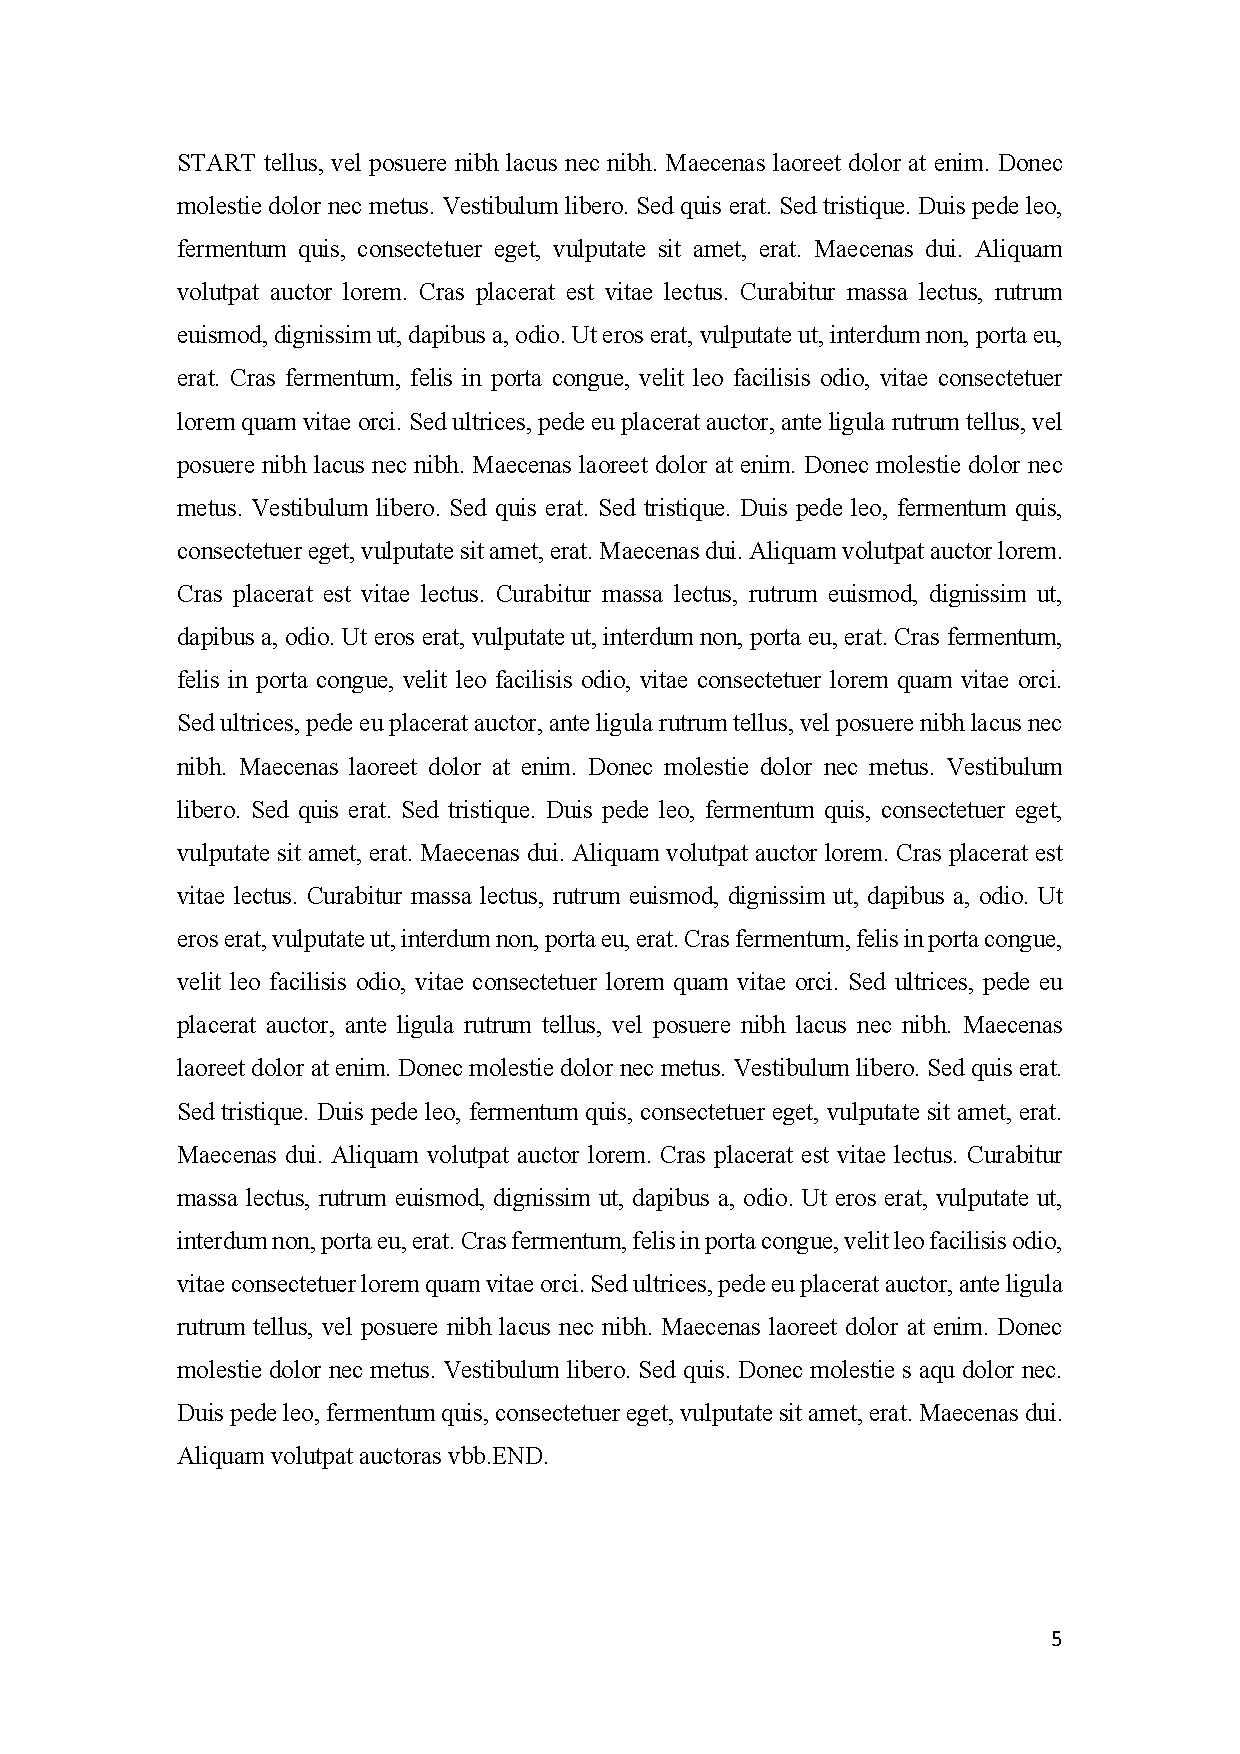
\includepdf[pages=-]{Anexos/uma folha doc 12pts.pdf}
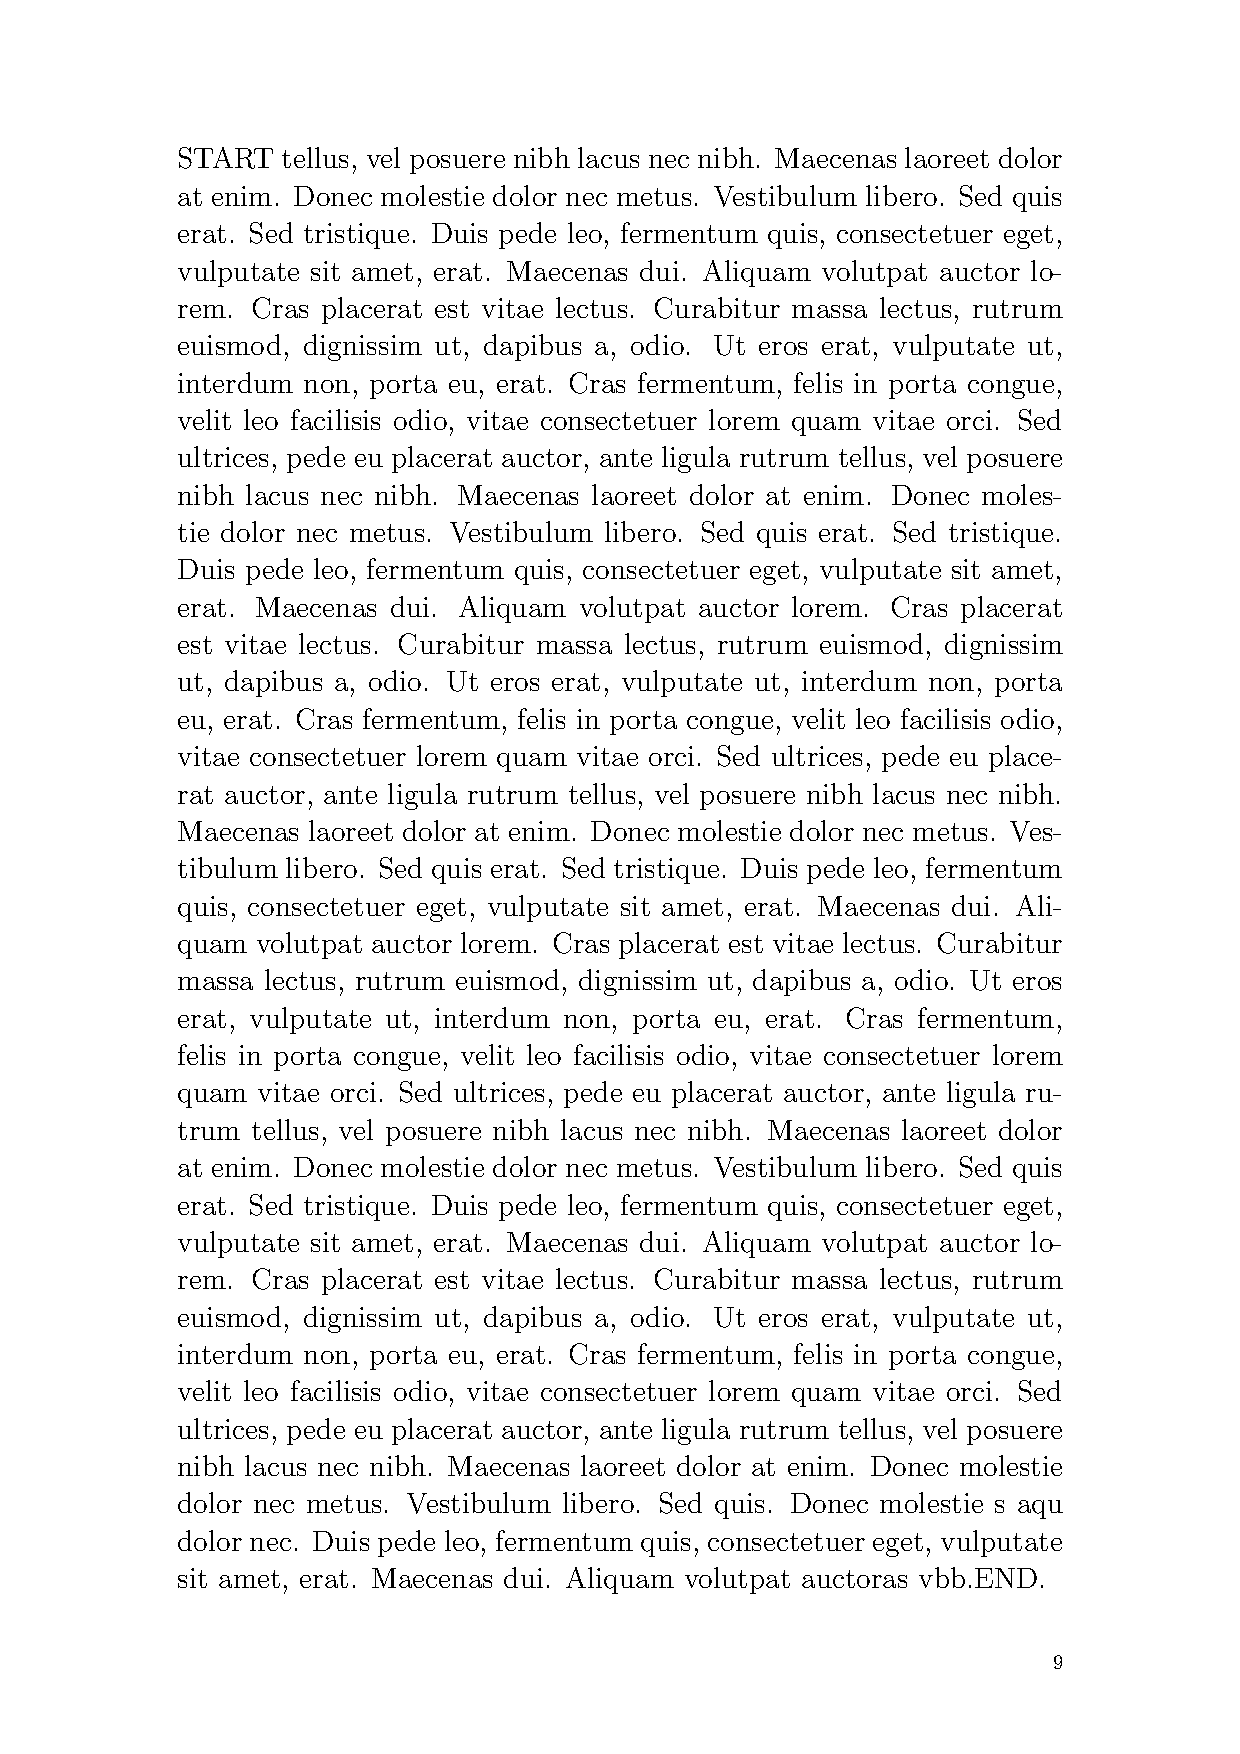
\includepdf[pages=-]{Anexos/uma folha latex 10pts class article.pdf}
\end{document}